% Created 2017-11-07 Tue 18:45
% Intended LaTeX compiler: pdflatex
\documentclass[titlepage]{article}
\usepackage[utf8]{inputenc}
\usepackage[T1]{fontenc}
\usepackage{graphicx}
\usepackage{grffile}
\usepackage{longtable}
\usepackage{wrapfig}
\usepackage{rotating}
\usepackage[normalem]{ulem}
\usepackage{amsmath}
\usepackage{textcomp}
\usepackage{amssymb}
\usepackage{capt-of}
\usepackage{hyperref}
\usepackage{mathptmx}
\setlength{\parindent}{2em}
\setlength{\parskip}{1em}
\author{Xiong ChenYu \\
U1521516C \\
EEE \\
}
\date{Oct. 20, 2017 \\
}
\title{
\includegraphics[width=\textwidth]{img/NTU.png} \\
[1\baselineskip] Report \\
On \\
EE4483/IM4483 \\
Artificial Intelligence and Data Mining \\
Continuous Assessment \\
BY FP growth \\
[2\baselineskip]}
\hypersetup{
 pdfauthor={Xiong ChenYu \\
U1521516C \\
EEE \\
},
 pdftitle={
\includegraphics[width=\textwidth]{img/NTU.png} \\
[1\baselineskip] Report \\
On \\
EE4483/IM4483 \\
Artificial Intelligence and Data Mining \\
Continuous Assessment \\
BY FP growth \\
[2\baselineskip]},
 pdfkeywords={},
 pdfsubject={},
 pdfcreator={Emacs 27.0.50 (Org mode 9.1.2)},
 pdflang={English}}
\begin{document}

\maketitle
\tableofcontents

\listoftables
\listoffigures

\newpage

\section{Abstract}
\label{sec:org24e01af}
This report answer questions of the research and study on the continues assessment.

\newpage

\section{Question 1 (How many frequent itemsets have the minimum support of 20\%, 10\%, 5\%, and 3\% respectively?)}
\label{sec:org3dfee9b}

In John Hughes’s model, their are 4 distinguishable
steps to constructing and evaluating the game tree: defining
the representation, generating the game tree, applying
and evaluating heuristics, and applying lazy evaluation to
the game tree generator. He defines these functions as prototypes
to illustrate how easy it is to compose higher-order
functions to form more powerful functions but does not explicitly
define the function.

I skip the game definition and leave the code in appendix.  I will explain the heuristic measure below.

\begin{figure}[htbp]
\caption{\label{fig:org0d4b9c5}
heuristics estimate}
\centering
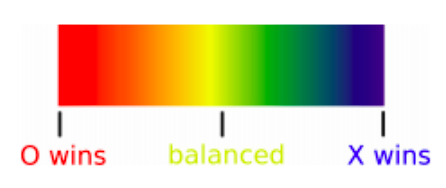
\includegraphics[width=10cm]{./img/color.png}
\end{figure}

  The heuristic rely heavily on game-specific knowledge. Finding good evaluation
heuristics is difficult.The heuristic measure I use for tic tac toe is like blow.

\begin{enumerate}
\item In this adversarial game. I define that the X will go for the maximum
marks. While O will go for the minimum marks.
\item I calculate the single mark for rows columns diagonal and anti-diagonal.
\item The single mark is define by the count difference of X pieces and O pieces
\begin{itemize}
\item If the count of X pieces minus the count of O pieces is 3, that means X wins, then get 1000.
\item If the count of X pieces minus the count of O pieces is 2, that means X
have 2 pieces while O have 0 in a line, then get 50.
\item If the count of X pieces minus the count of O pieces is -3, that means O wins, then get -1000.
\item If the count of X pieces minus the count of O pieces is -2, that means O
have 2 pieces while X have 0 in a line, then get -50.
\item otherwise 0 marks will be given.
\end{itemize}
\item Then add the single marks rows by rows, columns by columns, and the 2
diagonal together to get the final marks
\end{enumerate}

This evaluation heuristic can be applied to non-final positions of game state,
which can be future apply to the minimax search algorithm.

\begin{center}
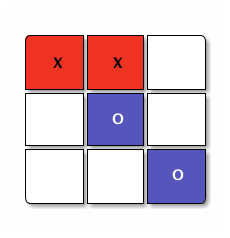
\includegraphics[width=.9\linewidth]{d.png}
\end{center}

For example this is a random game State. The total score is
\begin{multline}
   Total Score = row1 + row2 + row3 + column1 + column2 + column3 + diagonal +
anti-diagonal \\
               = 50 + 0 + 0 + 0 + 0 + 0 + 0 + 0 = 50
\end{multline}

\section{Question 2 (What are the respective percentages of frequent 3‐itemsets, and 2‐itemsets, with respect to all possible itemsets, which have a minimum support of 3\%?)}
\label{sec:org691986d}

The search strategy is minimax algorithm with Alpha-beta pruning to decrease
the number of nodes that are evaluated by the minimax algorithm in its search
tree.

With an (average or constant) branching factor of b, and a search depth of n
plies, the maximum number of leaf node positions evaluated (when the move
ordering is pessimal) is \(O(bb...*b)\) = \(O(b^n)\) – the same as a simple minimax
search. If the move ordering for the search is optimal (meaning the best moves
are always searched first), the number of leaf node positions evaluated is
about \(O(b*1*b*1*...*b)\) for odd depth and \(O(b*1*b*1*...*1)\) for even depth, or
\(O(b^\frac{n}{2})\). In the latter case, where the ply of a search is even, the
effective branching factor is reduced to its square root, or, equivalently,
the search can go twice as deep with the same amount of computation.

The explanation of \(b*1*b*1*\)\ldots{} is that all the first player's moves must be
studied to find the best one, but for each, only the best second player's move
is needed to refute all but the first (and best) first player move – alpha–beta
ensures no other second player moves need be considered.

\begin{figure}[htbp]
\caption{\label{fig:org0bcf242}
"Skip" every 2 level}
\centering
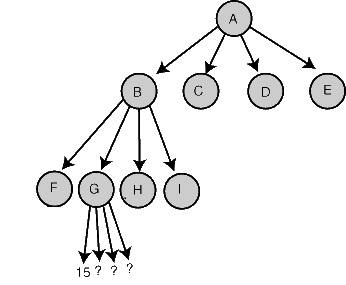
\includegraphics[width=10cm]{./img/alpha.png}
\end{figure}

The best case time complexity of Alpha-beta pruning is \(O(b^{\frac{n}{2}})\).
And the space complexity is the b*n.

\section{Question 3 (How many association rules have a minimum confidence of 50\% and a minimum support of 5\% and 10\%, respectively? Briefly explain how the minimum support affects the strong rules generated. )}
\label{sec:orga8cc08e}

By compare to other heuristic search algorithm. The Alpha-beta pruning is a
best choice balance between a greedy search algorithm and brute forth search
algorithm.

The greedy search algorithm runs fast compare to Alpha-beta pruning. The time
complexity is O(1) compare to Alpha-beta pruning which is \(O(b^{\frac{n}{2}})\). But it
have it's own shortage. The evaluation function for greedy search algorithm is
very hard to write. And if the evaluation function does not describe the game
model well. The greedy algorithm AI will easily get the local maximum rather
than global and lose the game.

And compare to another extreme, the brute forth search, which is very easy to
write the evaluation function, just 3 case win, lose or draw. And the program
will always get the global maximum and take the best strategy. But for the
simple game like Tic Tac Toe, the brute forth search is possible cause the
solution space is only \(9! = 362880\). But for other games like chess. It is
impossible. Actually, the chess computer Deep Blue (the first one to beat a
reigning world champion, Garry Kasparov at that time) looked ahead at least 12
plies, then applied a heuristic evaluation function. The searching function it
used is the Alpha-beta pruning.

By compare to the 2 extreme one is the fast but hard to write evaluation
function and easily get local maximum by using the greedy searching algorithm.
Another is the easiest evaluation but time consuming. The advantages of
minimax Alpha-beta pruning searching algorithm balance perfect between the
time consuming of running code and the time consuming of witting the
evaluation functions.

The limitations of using the minimum Alpha-beta pruning is that this searching
algorithm can only be use in the 2 person zero-sum adversarial game.

\section{Question 4 (List three association rules that have the highest support with 100\% confidence?)}
\label{sec:orgfb3770d}
If the pruning level is more then 5, then my program will always make the best move, so if I make one single mistake the program can win the game.

\section{Question 5 (Do you find any “interesting” rules? What are they? Briefly explain why.)}
\label{sec:orgc165414}
If the pruning level is more then 5, then my program will always make the best move, so if I make one single mistake the program can win the game.

\section{REFERENCE}
\label{sec:orgda6c45d}
[1] J. Hughes. Why functional programming matters. The
Computer Journal, 32(2):98–107, 1989. \\
\url{https://en.wikipedia.org/wiki/Minimax\#Minimax\_algorithm\_with\_alternate\_moves} \\
\url{https://en.wikipedia.org/wiki/Alpha\%E2\%80\%93beta\_pruning}       \\
\url{http://perugini.cps.udayton.edu/teaching/courses/Spring2016/cps499/projects/korenewychs1/korenewychs1-paper.pdf}

\section{APPENDIX A}
\label{sec:org1fd0978}
\begin{verbatim}
import Data.Array
import Data.List (intercalate, intersperse,elemIndex)
import Data.Tree

data Cell = B | X | O
  deriving (Enum, Read, Eq, Ord)

instance Show Cell where
  show B = "."
  show X    = "X"
  show O    = "O"

opposite :: Cell -> Cell
opposite B = B
opposite X = O
opposite O = X

type Position = (Int, Int)
type State = Array Position Cell

newGame :: State
newGame = listArray boardInds $ repeat B
        where boardInds = ((0,0), (2,2))

update :: State -> (Position, Cell) -> State
update st pc = st // [pc]

getTurn :: State -> Cell
getTurn st
  | pieceDiff == 0    = X
  | pieceDiff == 1    = O
  | otherwise = error "encountered invalid board state"
  where pieceDiff = (count X st) - (count O st)
        count cell state = length . filter (==cell) $ elems state

lookupCell :: State -> Position -> Cell
lookupCell = (!)

getRow, getCol :: State -> Int -> [Cell]
getRow s i = [ lookupCell s (i,j) | j <- [0,1,2] ]
getCol s i = [ lookupCell s (j,i) | j <- [0,1,2] ]

getDiag, getAntiDiag :: State -> [Cell]
getDiag s = [ lookupCell s (i,j) | (i,j) <- [(0,0), (1,1), (2,2)] ]
getAntiDiag s = [ lookupCell s (i,j) | (i,j) <- [(2,0), (1,1), (0,2)] ]

win :: Cell -> State -> Bool
win piece state = checkRows || checkCols || checkDiag || checkAntiDiag
  where checkWin piece list = all (==piece) list
        checkRows = any (==True) [checkWin piece $ getRow state i | i <- [0,1,2]]
        checkCols = any (==True) [checkWin piece $ getCol state i | i <- [0,1,2]]
        checkDiag = checkWin piece $ getDiag state
        checkAntiDiag = checkWin piece $ getAntiDiag state

draw :: State -> Bool
draw st = (length . filter (/=B) $ elems st) == 9

moves :: State -> [State]
moves st
  | win X st || win O st = []
  | otherwise = map (\p -> update st (p, getTurn st)) (freePositions st)
  where freePositions st = filter (\p -> st ! p == B) $ indices newGame


pprint :: State -> IO ()
pprint st = putStrLn $ pretty
         where chars = concat $ map show $ elems st
               rows = [0..2] >>= \i -> return $ take 3 (drop (3*i) chars)
               pretty = intercalate "\n" rows


generate :: State -> Tree State
generate = unfoldTree (\s -> (s, moves s))

prune :: Int -> Tree a -> Tree a
prune 0 t = Node (rootLabel t) []
prune n t = Node (rootLabel t) (map (prune (n-1)) (subForest t))

staticVal :: State -> Int
staticVal = marks

marks :: State -> Int
marks state = checkRows + checkCols + checkDiag + checkAntiDiag
  where getMarks list = case (count X list) - (count O list) of
                          3 -> 1000
                          2 -> 5
                          -2 -> -5
                          -3 -> -1000
                          _ -> 0
        checkRows = sum [getMarks $ getRow state i | i <- [0,1,2]]
        checkCols = sum [getMarks $ getCol state i | i <- [0,1,2]]
        checkDiag = getMarks $ getDiag state
        checkAntiDiag = getMarks $ getAntiDiag state
        count cell list = length . filter (==cell) $ list

mapmin :: Ord a => [[a]] -> [a]
mapmin [] = []
mapmin (xs:rest) = (omit n rest)
  where n = minimum xs
        omit n [] = [n]
        omit n (xs:rest) | minleq n xs = omit n rest
                         | otherwise   = omit k rest
                             where k = minimum xs
        minleq _ [] = False
        minleq n (y:ys) | y <= n = True
                        | otherwise = minleq n ys

mapmax :: Ord t => [[t]] -> [t]
mapmax [] = []
mapmax (xs:rest) = (omit n rest)
  where n = maximum xs
        omit n [] = [n]
        omit n (xs:rest) | maxleq n xs = omit n rest
                          | otherwise   = omit k rest
                              where k = maximum xs
        maxleq _ [] = False
        maxleq n (y:ys) | y >= n = True
                        | otherwise = maxleq n ys

abMaxList :: (Ord a) => Tree a -> [a]
abMaxList (Node x []) = [x]
abMaxList (Node x subs) = mapmin . map abMinList $ subs

abMinList :: (Ord a) => Tree a -> [a]
abMinList (Node x []) = [x]
abMinList (Node x subs) = mapmax . map abMaxList $ subs

minIndex :: Ord a => [a] -> Int
minIndex xs = head $ filter ((== minimum xs) . (xs !!)) [0..]

maxIndex :: Ord a => [a] -> Int
maxIndex xs = head $ filter ((== maximum xs) . (xs !!)) [0..]

abmax :: State -> Int
abmax = maximum .
        abMaxList .
        fmap staticVal .
        prune 4 .
        generate

abmin :: State -> Int
abmin = minimum .
           abMinList .
           fmap staticVal .
           prune 4 .
          generate

playX :: State -> State
playX s = moves s !! (maxIndex . fmap abmin $ moves s)

playO :: State -> State
playO s = moves s !! (minIndex . fmap abmax $ moves s)

playAi :: State -> State
playAi s = case getTurn s of
           X -> playX s
           _ -> playO s

playHuman :: State -> Position -> State
playHuman s p = update s (p,(getTurn s))

main :: IO ()
main = putStrLn "Welcome to the Heuristic Tic Tac Toe" >>
       putStrLn "Below show the board, the up left is the root" >>
       putStrLn "Please decide you want to play first or second (X or O)" >>
       fmap (read::String -> Cell) getLine >>= loop newGame

loop:: State -> Cell -> IO()
loop s c
    | c == X =
        if win O s then
            pprint s >>
            putStrLn "Owin"
          else
            if win X s then
                  pprint s >>
                  putStrLn "Xwin"
              else
                if draw s then
                    pprint s >>
                    putStrLn "Draw"
                else
                    pprint s >>
                    putStrLn "Please input as (x,y) such as (0,0) 0<=x<=2, 0<=y<=2" >>
                    fmap (read::String -> Position) getLine >>=
                    \p -> loop  (playHuman s p) (opposite  c)
    | otherwise =
        if win O s then
            pprint s >>
            putStrLn "Owin"
          else
            if win X s then
                  pprint s >>
                  putStrLn "Xwin"
              else
                if draw s then
                    pprint s >>
                    putStrLn "Draw"
                else
                  pprint s >>
                  putStrLn "Now please wait AI to calculate" >>
                  loop (playAi s) (opposite c)
\end{verbatim}
\end{document}